\documentclass[openany]{article}
\usepackage[a4paper,margin=1in,bottom=1.5in]{geometry} % define margins. Bottom margin is used to lift a little bit the page number.
\usepackage[english]{babel} % document language is english
\usepackage{tikz} % for drawing (currently not used).
\usepackage{graphicx} % for including images
\usepackage[export]{adjustbox}
\usepackage{fancyhdr} % used for creating headers and footers. only used in title page in this document.
\usepackage{tabularx} % creation of more complex tables
\usepackage{array} % allow elements of tabular environment to have vertical alignment, e.g., center alignment.
\usepackage{nameref} % make it possible to reference by name
\usepackage{hyperref} % allow hiperlinks (links to other document parts and extern links)
\usepackage{etoc} % used for generation of section local table of contents
\usepackage{placeins}

% Define graphics path
\graphicspath{{figs/}}

% Configure the cross reference hyper links color
\hypersetup{
    colorlinks=true,
    linkcolor=blue,
}

\newcolumntype{C}{>{\centering\arraybackslash}X} % new column type for tabularx
						 % centered (\centering), adjust width in order to fill table width (X type)

% Configure header in 'titlepage'
\pagestyle{fancy}
\lhead{
\includegraphics[width=4.5cm]{logo_cnpem}}
\rhead{
\includegraphics[width=4cm]{logo_lnls}}
\renewcommand{\headrulewidth}{0pt}
\setlength{\headheight}{52pt}
% Clean footer
\fancyfoot{}

% increase table height factor a little bit (taller cells)
\renewcommand{\arraystretch}{1.5}

%==== Begin DOCUMENT ====
\begin{document}

%--- Begin title page ---
\begin{titlepage}

% Add header to this page
\thispagestyle{fancy}

% Center elements
\begin{center}

% title of title page
\topskip0pt % perfectly centered
\vspace*{\fill}
\textbf{\Huge STD-EVE Hardware Manual}\\[20pt]
\textbf{\Huge Version 1.0}\\[20pt]
\textbf{\Huge February/2017}
\vspace*{\fill}

% footer of title page
\vfill
\textbf{Beam Diagnostics Group (DIG)}\\[5pt]
\textbf{Brazilian Synchrotron Light Laboratory (LNLS)}\\[5pt]
\textbf{Brazilian Center for Research in Energy and Materials (CNPEM)}
\end{center}

\end{titlepage}
%--- End of title page ---

\newpage
\pagestyle{plain} % restore default page style

%--- About this manual ---
\paragraph{}{\Large\bfseries About this manual}

\paragraph{} This manual is intended for people who need information about the STD-EVE hardware. Information about the timing system structure and operation, firmware, or software can be found in the corresponding manuals.

%--- Table of contents ---
\tableofcontents

\newpage
%--- Section: Hardware Specification ---
\section{Hardware Specification}

\par STD-EVE is a 19 inches 1U module. \\ 110/220V 50/60Hz AC power supply.

% EVE figure
\begin{figure}[!h]
\caption{STD-EVE}
\label{fig:std-eve}
\centering
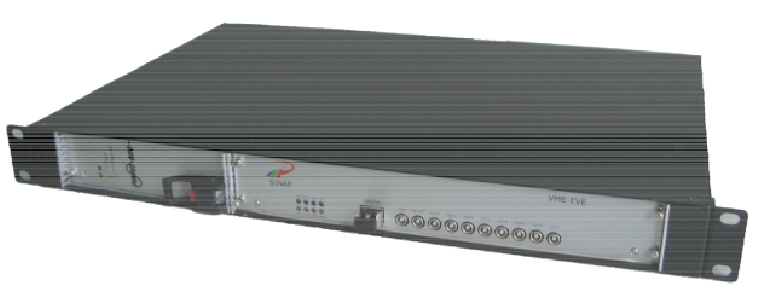
\includegraphics[width=0.7\textwidth]{std-eve-image}
\end{figure}

	% Specification table - Connectors - front panel
	\begin{table}[!h]
	  \centering
	  \caption{STD-EVE front panel connectors}
	  \label{tab:front-panel-connectors}
	  \begin{tabular}{| m{3.5cm} m{4.0cm} m{7.0cm} |}
	    \hline
	    \bfseries Connector & \bfseries Type & \bfseries Description / Specification \\ \hline
	    UPLINK & LC Duplex & Fiber for uplink \\ \hline
	    INH & LEMO EPL.00.250.NTN & \begin{tabular}{@{}m{6cm}@{}}
					Interlock input \\
	    				TTL level \\
	    				50ohm input impedance
					\end{tabular} \\ \hline
	    RF OUT & LEMO EPL.00.250.NTN RF & \begin{tabular}{@{}m{6cm}@{}}
					      Recovery clock output \\
	    				      Square waveform \\
	    				      -3dBm (0.23V peak)
					      \end{tabular} \\ \hline
	    OUT0 - OUT7 & LEMO EPL.00.250.NTN & 3.3V LVTTL level \\ \hline	   
	  \end{tabular}
	\end{table}

	% Specification table - LEDs - front panel
	\begin{table}[!h]
	  \centering
	  \caption{STD-EVE front panel LEDs}
	  \label{tab:front-panel-leds}
	  \begin{tabular}{| m{3.5cm} m{4.0cm} m{7.0cm} |}
	    \hline
	    \bfseries LED & \bfseries Type & \bfseries Description / Specification \\ \hline
	    EVG & Green LED & Always Off \\ \hline
	    EVR & Green LED & Always On \\ \hline
	    FOUT & Green LED & Always Off \\ \hline
	    FPGA & Green LED & FPGA downloaded \\ \hline
	    INH & Red LED & Interlock input activated \\ \hline
	    ENA & Green LED & STD-EVE enabled \\ \hline
	    EVT & Yellow LED & (Blink) Event code received \\ \hline
	    LINK & Green LED & Uplink established \\ \hline
	  \end{tabular}
	\end{table}

	% Specification table - Connectors - rear panel
	\begin{table}[!h]
	  \centering
	  \caption{STD-EVE rear panel connectors}
	  \label{tab:rear-panel-connectors}
	  \begin{tabular}{| m{3.5cm} m{4.0cm} m{7.0cm} |}
	    \hline
	    \bfseries Connector & \bfseries Type & \bfseries Description / Specification \\ \hline
	    ETHERNET & RJ45 & 10/100Mbit Ethernet port \\ \hline
	    RST & Button & Reset Ethernet \\ \hline
	  \end{tabular}
	\end{table}

	% Specification table - LEDs - rear panel
	\begin{table}[!h]
	  \centering
	  \caption{STD-EVE rear panel LEDs}
	  \label{tab:rear-panel-leds}
	  \begin{tabular}{| m{3.5cm} m{4.0cm} m{7.0cm} |}
	    \hline
	    \bfseries LED & \bfseries Type & \bfseries Description / Specification \\ \hline
	    PWR & Green LED & Power on \\ \hline
	  \end{tabular}
	\end{table}

\FloatBarrier
%--- Section: STD-EVE Hardware ---
\section{STD-EVE Hardware Functions}

		\paragraph{} The STD-EVE module is an \emph{Event Receiver} (front panel green LED \emph{EVR} is always on). In order to distinguish it from the STD-EVO/EVR (STD-EVO configured as EVR), it is going to be referred to as EVE. The role of an \emph{Event Receiver} is to convert the data frames broadcast by the \emph{Event Generator} (EVG) into trigger and clock signals that can be transmitted to devices in the accelerator. The STD-EVE module has two inputs in the front panel, which are: \emph{UPLINK}, and \emph{INH}. The signal associated with each input is described below.

		\paragraph{} The \emph{UPLINK} input is connected to one of the EVG's SFP outputs (generally with fiber optic cables). This input receives data frames broadcast by the EVG containing timing information to be converted into triggers and clocks.
		\paragraph{} The \emph{INH} input is an interlock active-low input.
		\paragraph{} The Timing System data frame is composed of two parts of 8 bits each: the event code, which is converted by the EVE into a trigger, and the \emph{Distributed Bus} (\emph{DBUS}), which carries information of 8 different clocks (see figure \ref{fig:data-frame-eve}). The parallel frequency for transmission of data frames by the EVG is defined by the EVG's \emph{event clock}, which is a submultiple of the RF frequency. In addition to obtaining the event code and \emph{Distributed Bus} clocks, the \emph{Event Receiver} uses the received data frames to recover the \emph{event clock} and lock itself to the EVG's reference clock.

		\begin{figure}[!h]
		\begin{tabular}{|cccccccc|c|c|c|c|c|c|c|c|}
		\hline
		\multicolumn{8}{|c|}{\emph{Event code}} & \multicolumn{8}{c|}{\emph{DBus}} \\ \hline
		\multicolumn{8}{|c|}{8 bits} & 7 & 6 & 5 & 4 & 3 & 2 & 1 & 0 \\ \hline
		\end{tabular}
		\centering
		\caption{Timing System Data Frame}
		\label{fig:data-frame-eve}
		\end{figure}
\FloatBarrier


		\paragraph{} The EVE has 8 electrical outputs in the front panel (OUT0 - OUT7). Each OUTx can be configured to output one of the \emph{Distributed Bus} clocks, or transmit one of the configured triggers.
		\paragraph{} The EVE triggers are configured through 24 independent channels (OTP channels). Each OTP channel can be configured to generate a trigger in response to the reception of a given event. The OTP channel also has other parameters, which define the characteristics of the output trigger, i.e., delay, width, polarity, and number of pulses.
		\paragraph{} The \emph{Event Receiver} has timestamping functinality. It has a timestamp register containing the current UTC timestamp, which is incremented through special event codes, or the \emph{Distributed Bus} bit 6 (DBUS 6) clock, depending on the configuration. The timestamp register contains a subsecond counter as well. This counter is updated by the \emph{event clock} recovered from the \emph{UPLINK}. The module has also a timestamp FIFO for storing event codes and the timestamp in which they were received. The \emph{OTP channels} have a parameter which tells whether the event being monitored should be stored upon reception.
		\paragraph{} Details of the EVE submodules are provided later in this section.

		\subsubsection{Clock Recovery}\label{sec:eve-clock-recovery}

			\paragraph{} The \emph{Event Generator} broadcasts the event code and \emph{Distributed Bus} data frame every event clock period, even when there is no event scheduled, in which case a dummy event with code 0 is broadcast. The data frame is broadcast using 8b10b encoding (see figure \ref{fig:encoding-decoding}). The \emph{Event Receivers} use the data frames that arrive from the \emph{UPLINK} to recover the \emph{event clock}.

			% Encoding-decoding figure
			\begin{figure}[!h]
			\caption{Timing system encoding-decoding scheme}
			\label{fig:encoding-decoding}
			\centering
			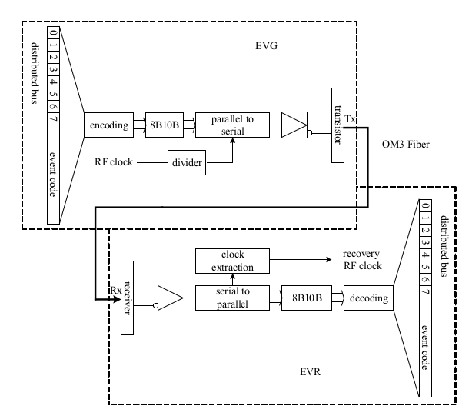
\includegraphics[width=0.7\textwidth]{encoding-decoding-image}
			\end{figure}
\FloatBarrier

		\subsubsection{Trigger Generation}\label{sec:eve-trigger-generation}

			\paragraph{} The EVE has 24 \emph{OTP} channels, each of which can be configured to generate a trigger upon the reception of a given event. The OTP channels parameters are configured in the \nameref{reg:eve-otp}.
			The \emph{EVT} parameter specifies the event code responsible for generating the trigger.
			The \emph{DELAY} parameter specifies the delay between the event reception and the output trigger in \emph{event clock} period units.
			The \emph{WIDTH} parameter specifies the width of the pulse generated in \emph{event clock} period units.
			The \emph{POL} parameter specifies the pulse polarity.
			The \emph{PULSES} parameter specifies the number of pulses to be generated in response to the event reception. When \emph{PULSES} is greater than one, the trigger generated is in fact a pulse train. The pulse train period is 2 times \emph{WIDTH} and the duty cycle is 0.5.
			\paragraph{} The EVE's \emph{Timestamp FIFO} can store the instant when some event is received. Each \emph{OTP} channel has a \emph{TIME} parameter that enables the timestamping function for the event code being monitored.

		\subsubsection{FP Ouputs}\label{sec:eve-fp-outputs}

			\paragraph{} The FP outputs correspond to the OUT0 - OUT7 outputs in the EVE front panel. The OUT0 - OUT7 outputs can be configured in the \nameref{reg:eve-out}. The \emph{OUTx} signal source can be mapped to one of the \emph{OTP} channels, or any of the \emph{Distributed Bus} clocks. The source selection is defined by the \emph{SEL} parameter.
			\par The \emph{ITL} parameter enables/disables the interlock function for the corresponding \emph{OUT} channel. When the \emph{OUTx} channel has ITL \emph{enabled}, the channel is inhibited whenever the EVE's interlock input (\emph{INH}) is active (active-low signal).
			\paragraph{} The OUTx signal has an associated RF delay (\emph{RFDLY}) and fine delay (\emph{FINEDLY}). The RF delay resolution is \(\frac{1}{20}\) of \emph{event clock} period. When the value of \emph{RFDLY} is set to 31, the RF delay of the OUTx output is set by the EVG's \emph{Event Sequencer} special event codes 0x40 - 0x53, which set the delay value from 0 to 19 respectively. The RF delay special event codes can be written to the EVG's \emph{Sequence RAM}, in order to give event timestamps enough resolution to, for example, allow single bucket injection. The fine delay resolution is 5ps, and may be used for fine adjustment of the trigger timing.

		\subsubsection{RF Ouput}\label{sec:eve-rf-output}

			The EVE's \emph{RF OUT} output in the front panel is able to provide a square waveform with frequency multiple of the recovered \emph{event clock}. The \emph{RF OUT} can be configured to output x1, x2, x4, x5, and x10 the \emph{event clock}. The \emph{RF OUT} settings are defined in the \nameref{reg:eve-rf-output}.

		\subsubsection{Timestamp}\label{sec:eve-timestamp}
		
			\paragraph{} The EVE has timestamping function, which allows it to register when events of interest are received. To this end, the module maintains a timestamp register containing the 64-bit Timing System timestamp, which comprises a 32-bit \emph{UTC} timestamp and a 32-bit \emph{SUBSECOND} timestamp. The EVG sets the EVE's timestamp (generally once), and then increments it every second. The timestamp settings and status can be accessed in the \nameref{reg:eve-timestamp}.
			\paragraph{} The 32-bit \emph{UTC} timestamp stores the number of seconds passed since some epoch. This value can only be modified by a timestamp broadcast. When the EVG broadcasts its UTC timestamp, the EVE first receives the special event code 0x74. The event 0x74 resets the \emph{SUBSECOND} counter and tells the EVE to treat the next 4 events as UTC information, instead of actual event codes. The UTC information received then replaces the current 4-byte \emph{UTC} value.
			\paragraph{} The \emph{SUBSECOND} counter is incremented by the recovered \emph{event clock}, providing \emph{event clock} period resolution to the timestamp.
			\paragraph{} The \emph{TIMESRC} field specifies the PPS source, i.e., the signal which is going to increment the EVE's UTC. When \emph{TIMESRC} is configured as \emph{EVENT}, the \emph{UTC} field is incremented by the special event 0x73, which is sent at the start of every second. When the \emph{TIMESRC} is configured as \emph{DBUS}, the \emph{UTC} field is incremented by the \emph{DBUS 6} clock. When \emph{TIMESRC} is \emph{INTERNAL}, the internal oscillator provides the increment signal. Once a PPS is received, the \emph{SUBSECOND} counter is reset and the \emph{UTC} timestamp is incremented.
			\paragraph{} In addition to the timestamp special events already mentioned, there are also event code 0x71, which resets the \emph{SUBSECOND} timestamp, and event code 0x72, which resets the \emph{UTC} timestamp.

			\paragraph{Timestamp FIFO} The EVE has a \emph{Timestamp FIFO}, also referred to as \emph{Timestamp Log}, capable of storing 16384 sets of event code and timestamp (32-bit \emph{UTC} and 32-bit \emph{SUBSECOND}). The purpose of the \emph{Timestamp Log} is to store the instant when relevant events are received. The \nameref{reg:eve-timestamp-log} is used to read and command the \emph{Timestamp FIFO}. Each \hyperref[sec:eve-trigger-generation]{OTP channel} has a timestamping setting, defining whether the event code mapped to that channel should be stored along with its timestamp once received.
			\paragraph{} The \emph{Timestamp FIFO} operates as a circular buffer, replacing the oldest timestamp value by the newest, in the case that the FIFO is full and a new timestamp is stored.
			The \emph{EMPTY} and \emph{FULL} flags indicate when the FIFO is empty, or full respectively.
			\paragraph{} Writing to the \emph{PULL} field pulls the \emph{Timestamp Log} oldest value. Reading \emph{PULL} has no effect. The pull action updates the \emph{Timestamp Log}'s \emph{UTC}, \emph{SUBSECOND}, and \emph{EVENT} fields with the UTC, subsecond, and event code obtained from the \emph{Timestamp FIFO}. The pulled information is erased from the Log. The procedure for reading the \emph{Timestamp Log} consists of writing to \emph{PULL} and reading the Log's \emph{UTC}, \emph{SUBSECOND}, and \emph{EVENT} fields.
			\paragraph{} The \emph{LOGCOUNT} field indicates how many sets of event code and timestamp are stored in the \emph{Timestamp FIFO}.
			The \emph{RSTLOG} field resets the \emph{Timestamp FIFO}, i.e., clear all stored values. The \emph{STOPLOG} field stops the timestamping function while set. Both \emph{RSTLOG} and \emph{STOPLOG} return their current value when read.

		\subsubsection{Registers}\label{sec:eve-registers}

			\begin{center}
			\renewcommand{\arraystretch}{3} % valid only in this 'center' environment
			\begin{tabular}{p{2cm} p{5cm} p{7cm}}
			\bfseries Address & \bfseries Register Name & \bfseries Description \\ \hline
			\bfseries 0 & \nameref{reg:eve-control-status} & General settings and status. Enable/disable module, \emph{UPLINK} status, and interlock input status. \\ \hline
			\bfseries 1-16 & \nameref{reg:eve-otp} & OTPx settings. Specifies OTPx trigger delay, width, polarity, number of pulses, and mapped event. Also enables/disables timestamping option. \\ \hline
			\bfseries 17-24 & \nameref{reg:eve-out} & OUTx settings. Specifies OUTx output signal source, RF delay, and fine delay. Also enables/disables the interlock function for the channel being configured. \\ \hline
			\bfseries 25 & \nameref{reg:eve-rf-output} & RF ouput (\emph{RF OUT}) settings. Specify the RF output multiplier. \\ \hline
			\bfseries 51 & \nameref{reg:eve-timestamp} & Timestamp information and settings. Define PPS signal source, reading of \emph{UTC} and \emph{SUBSECOND} values.  \\ \hline
			\bfseries 52 & \nameref{reg:eve-timestamp-log} & Timestamp Log settings. \emph{Timestamp FIFO} reading and commanding. \\ \hline
			\bfseries 62 & \nameref{reg:eve-firmware-version} & 12-byte code for current firmware version. \\ \hline
			\bfseries 63 & \nameref{reg:eve-configuration} & Main STD-EVO configuration options. Alive counter, and \emph{Clock mode} setting. \\ \hline
			\end{tabular}
			\end{center}
	
			\paragraph{Control and Status Register}\label{reg:eve-control-status}{\large\bfseries [0]}

				% Reg C
				\paragraph{}{\large RegC}
				% bits 15-8
				\begin{center}
				\begin{tabularx}{0.9\textwidth}{C C C C C C C C}
				Bit 15 & Bit 14 & Bit 13 & Bit 12 & Bit 11 & Bit 10 & Bit 9 & Bit 8 \\
				% fields
				\hline
				\multicolumn{1}{|c}{LINK} & \multicolumn{1}{|c|}{INHS} & & & & & & \multicolumn{1}{c|}{} \\ \hline
		    		\end{tabularx}
				\end{center}

				\begin{center}
				% bits 7-0
				\begin{tabularx}{0.9\textwidth}{C C C C C C C C}
				Bit 7 & Bit 6 & Bit 5 & Bit 4 & Bit 3 & Bit 2 & Bit 1 & Bit 0 \\
				% fields
				\hline
				\multicolumn{1}{|c}{} & & & & & & & \multicolumn{1}{|c|}{EVREN} \\ \hline
		    		\end{tabularx}
				\end{center}

				% Register fields description
				\bigskip
				\begin{tabular}{p{2.2cm} p{11.8cm}}
				EVREN & Enable/Disable EVE. Disabling the EVE disables all of its outputs. \\
				& \begin{tabular}{l l}
				0 & Disable \\
				1 & Enable \\
				\end{tabular} \\
				INHS & Interlock input status. The interlock input status only affects the OUTx outpus whose interlock function is enabled. \\
				& \begin{tabular}{l l}
				  0 & Disserted \\
				  1 & Asserted \\
				  \end{tabular} \\
				LINK & \emph{UPLINK} status. \\
				& \begin{tabular}{l l}
				  0 & Unlink \\
				  1 & Link \\
				  \end{tabular} \\
				\end{tabular}

			\paragraph{OTPx Register}\label{reg:eve-otp}{\large\bfseries [1-16]}

				\paragraph{}{\color{red} OTP0 - OTP15: Address 1 - 16}
				\paragraph{}{\color{red} OTP16 - OTP23: Address 25 - 32}

				% Reg A
				\paragraph{}{\large RegA}
				% bits 31-24
				\begin{center}
				\begin{tabularx}{0.9\textwidth}{C C C C C C C C}
				Bit 31 & Bit 30 & Bit 29 & Bit 28 & Bit 27 & Bit 26 & Bit 25 & Bit 24 \\
				% fields
				\hline
				\multicolumn{1}{|c}{EN} & \multicolumn{1}{|c}{POL} & \multicolumn{1}{|c|}{TIME} & & & & & \multicolumn{1}{c|}{} \\ \hline
		    		\end{tabularx}
				\end{center}
				
				\begin{center}
				% bits 23-16
				\begin{tabularx}{0.9\textwidth}{C C C C C C C C}
				Bit 23 & & & & & & & Bit 16 \\
				% fields
				\hline
				\multicolumn{8}{|c|}{PULSES} \\ \hline
		    		\end{tabularx}
				\end{center}

				\begin{center}
				% bits 15-8
				\begin{tabularx}{0.9\textwidth}{C C C C C C C C}
				Bit 15 & & & & & & & Bit 8 \\
				% fields
				\hline
				\multicolumn{8}{|c|}{PULSES} \\ \hline
		    		\end{tabularx}
				\end{center}

				\begin{center}
				% bits 7-0
				\begin{tabularx}{0.9\textwidth}{C C C C C C C C}
				Bit 7 & & & & & & & Bit 0 \\
				% fields
				\hline
				\multicolumn{8}{|c|}{EVT} \\ \hline
		    		\end{tabularx}
				\end{center}

				% Reg B
				\paragraph{}{\large RegB}
				\begin{center}
				% bits 31-0
				\begin{tabularx}{0.9\textwidth}{C C C C C C C C}
				Bit 31 & & & & & & & Bit 0 \\
				% fields
				\hline
				\multicolumn{8}{|c|}{DELAY} \\ \hline
		    		\end{tabularx}
				\end{center}

				% Reg C
				\paragraph{}{\large RegC}
				\begin{center}
				% bits 31-0
				\begin{tabularx}{0.9\textwidth}{C C C C C C C C}
				Bit 31 & & & & & & & Bit 0 \\
				% fields
				\hline
				\multicolumn{8}{|c|}{WIDTH} \\ \hline
		    		\end{tabularx}
				\end{center}

				% Register fields description
				\bigskip
				\begin{tabular}{p{2.2cm} p{11.8cm}}
				EN & Enable/Disable OTPx. Disabling the OTPx channel does not disable its timestamping function. \\
				& \begin{tabular}{l l}
				0 & Disable \\
				1 & Enable \\
				\end{tabular} \\
				POL & OTPx polarity. Specify the polarity of the OTPx output trigger. \\
				& \begin{tabular}{l l}
				0 & Normal \\
				1 & Inverted \\
				\end{tabular} \\
				TIME & Enable/Disable OTPx timestamping. When enabled, once the mapped event is received, the corresponding code and timestamp are stored in the \emph{Timestamp FIFO}. \\
				& \begin{tabular}{l l}
				0 & Timestamping \\
				1 & Not timestamping \\
				\end{tabular} \\
				PULSES & OTPx number of pulses. Specify the number of pulses to be generated. When the number of pulses is greater than 1, the output is a pulse train with duty cycle 0.5. \\
				EVT & OTPx mapped event. Specify the event to generate the trigger. \\
				DELAY & OTPx delay. Specify the delay between the reception of the mapped event and the trigger output. \\
				WIDTH & OTPx width. Specify the width of the trigger/pulse train pulse(s). \\
				\end{tabular}

			\paragraph{OUTx Register}\label{reg:eve-out}{\large\bfseries [17-24]}

				% Reg A
				\paragraph{}{\large RegA}
				% bits 31-24
				\begin{center}
				\begin{tabularx}{0.9\textwidth}{C C C C C C C C}
				Bit 31 & Bit 30 & Bit 29 & Bit 28 & Bit 27 & Bit 26 & Bit 25 & Bit 24 \\
				% fields
				\hline
				\multicolumn{1}{|c|}{ITL} & & & & & & & \multicolumn{1}{c|}{} \\ \hline
		    		\end{tabularx}
				\end{center}
				
				\begin{center}
				% bits 23-16
				\begin{tabularx}{0.9\textwidth}{C C C C C C C C}
				Bit 23 & & & & & & & Bit 16 \\
				% fields
				\hline
				\multicolumn{8}{|c|}{} \\ \hline
		    		\end{tabularx}
				\end{center}

				\begin{center}
				% bits 15-8
				\begin{tabularx}{0.9\textwidth}{C C C C C C C C}
				Bit 15 & & & & & & & Bit 8 \\
				% fields
				\hline
				\multicolumn{8}{|c|}{} \\ \hline
		    		\end{tabularx}
				\end{center}

				\begin{center}
				% bits 7-0
				\begin{tabularx}{0.9\textwidth}{C C C C C C C C}
				Bit 7 & Bit 6 & Bit 5 & Bit 4 & Bit 3 & Bit 2 & Bit 1 & Bit 0 \\
				% fields
				\hline
				\multicolumn{1}{|c}{} & \multicolumn{7}{|c|}{SEL} \\ \hline
		    		\end{tabularx}
				\end{center}

				% Reg B
				\paragraph{}{\large RegB}	
				\begin{center}
				% bits 15-8
				\begin{tabularx}{0.9\textwidth}{C C C C C C C C}
				Bit 15 & Bit 14 & Bit 13 & Bit 12 & Bit 11 & Bit 10 & Bit 9 & Bit 8 \\
				% fields
				\hline
				\multicolumn{1}{|c}{} & & & & & & \multicolumn{2}{|c|}{FINEDLY} \\ \hline
		    		\end{tabularx}
				\end{center}

				\begin{center}
				% bits 7-0
				\begin{tabularx}{0.9\textwidth}{C C C C C C C C}
				Bit 7 & & & & & & & Bit 0 \\
				% fields
				\hline
				\multicolumn{8}{|c|}{FINEDLY} \\ \hline
		    		\end{tabularx}
				\end{center}

				% Reg C
				\paragraph{}{\large RegC}
				\begin{center}
				% bits 7-0
				\begin{tabularx}{0.9\textwidth}{C C C C C C C C}
				Bit 7 & Bit 6 & Bit 5 & Bit 4 & Bit 3 & Bit 2 & Bit 1 & Bit 0 \\
				% fields
				\hline
				\multicolumn{1}{|c}{} & & & \multicolumn{5}{|c|}{RFDLY} \\ \hline
		    		\end{tabularx}
				\end{center}

				% Register fields description
				\bigskip
				\begin{tabular}{p{2.2cm} p{11.8cm}}
				ITL & Enable/Disable OUTx interlock function. When the interlock function is enabled, the OUTx will be inhibited while the EVE interlock input (\emph{INH}) is active. \\
				& \begin{tabular}{l l}
				  0 & Disable \\
				  1 & Enable \\
				  \end{tabular} \\
				SEL & OUTx source selection. Specifies the source of the OUTx signal from one of the \emph{OTP} channels or \emph{Distributed Bus} clocks. \\
				  & \begin{tabular}{l l}
				  0x10 - 0x1F & OTP0 - OTP15 \\
				  0x20 - 0x27 & Dbus0 - Dbus7 \\
				  0x30 - 0x37 & OTP16 - OTP23 \\
				  \end{tabular} \\
				FINEDLY & OUTx fine delay. The fine delay between the event code reception and the OUTx trigger. The fine delay unit is 5ps. \\
				RFDLY & OUTx RF delay. The RF delay between the event code reception and the OUTx trigger. The RF delay unit is \(\frac{1}{20}\) of \emph{event clock} period. When \emph{RFDLY} is set to 31, the delay is defined by \emph{Event Sequencer} event codes 0x40 - 0x53, which set the RF delay to 0 - 19, respectively. \\
				\end{tabular}

			\paragraph{RF Output Register}\label{reg:eve-rf-output}{\large\bfseries [25]}

				% Reg C
				\paragraph{}{\large RegC}
				% bits 7-0
				\begin{center}
				\begin{tabularx}{0.9\textwidth}{C C C C C C C C}
				Bit 7 & Bit 6 & Bit 5 & Bit 4 & Bit 3 & Bit 2 & Bit 1 & Bit 0 \\
				% fields
				\hline
				\multicolumn{1}{|c}{} & & & & & & & \multicolumn{1}{|c|}{CMSEL} \\ \hline
		    		\end{tabularx}
				\end{center}

				% Register fields description
				\bigskip
				\begin{tabular}{p{2.2cm} p{11.8cm}}
				CMSEL & RF output multiplier. Configuration of the \emph{RF OUT} output clock frequency, which is a multiple of the recovered \emph{event clock}. \\
				& \begin{tabular}{l l}
				0 & Disable \\
				1 & x1 \\
				2 & x2 \\
				3 & x4 \\
				4 & x5 \\
				5 & x10 \\
				\end{tabular} \\
				\end{tabular}

			\paragraph{Timestamp Register}\label{reg:eve-timestamp}{\large\bfseries [51]}

				% Reg A
				\paragraph{}{\large RegA}
				\begin{center}
				% bits 31-0
				\begin{tabularx}{0.9\textwidth}{C C C C C C C C}
				Bit 31 & & & & & & & Bit 0 \\
				% fields
				\hline
				\multicolumn{8}{|c|}{UTC} \\ \hline
		    		\end{tabularx}
				\end{center}

				% Reg B
				\paragraph{}{\large RegB}
				\begin{center}
				% bits 31-0
				\begin{tabularx}{0.9\textwidth}{C C C C C C C C}
				Bit 31 & & & & & & & Bit 0 \\
				% fields
				\hline
				\multicolumn{8}{|c|}{SUBSECOND} \\ \hline
		    		\end{tabularx}
				\end{center}

				% Reg C
				\paragraph{}{\large RegC}
				\begin{center}
				% bits 7-0
				\begin{tabularx}{0.9\textwidth}{C C C C C C C C}
				Bit 7 & Bit 6 & Bit 5 & Bit 4 & Bit 3 & Bit 2 & Bit 1 & Bit 0 \\
				% fields
				\hline
				\multicolumn{1}{|c}{} & & & & & & \multicolumn{2}{|c|}{TIMESRC} \\ \hline
		    		\end{tabularx}
				\end{center}

				% Register fields description
				\bigskip
				\begin{tabular}{p{2.2cm} p{11.8cm}}
				UTC & The timestamp UTC field, which is a 32-bit counter to store the number of seconds passed since some epoch. The counter is incremented by the source defined in \emph{TIMESRC}. The UTC can only be modified by EVG timestamp broadcasts or PPS signal. \\
				SUBSECOND & The timestamp subsecond field, which is a 32-bit counter to store the subsecond portion of the Timing System timestamp. SUBSECOND is incremented by the recovered \emph{event clock}, and thus, it has \emph{event clock} period resolution. The SUBSECOND is reset whenever a PPS signal or UTC broadcast is received. \\
				TIMESRC & The Pulse-per-second signal source, which is responsible for incrementing the timestamp UTC. The PPS signal can be obtained from the clock transmitted by the \emph{Distributed Bus} bit 6, from the special event code 0x73, which is broadcast by the EVG at the start of every second, or from the internal oscillator. \\
				& \begin{tabular}{l l}
				0 & Idle \\
				1 & DBUS (DBUS6) \\
				2 & Event \\
				3 & Internal \\
				\end{tabular} \\
				\end{tabular}

			\paragraph{Timestamp Log Register}\label{reg:eve-timestamp-log}{\large\bfseries [52]}

				% Reg A
				\paragraph{}{\large RegA}
				\begin{center}
				% bits 31-0
				\begin{tabularx}{0.9\textwidth}{C C C C C C C C}
				Bit 31 & & & & & & & Bit 0 \\
				% fields
				\hline
				\multicolumn{8}{|c|}{UTC} \\ \hline
		    		\end{tabularx}
				\end{center}

				% Reg B
				\paragraph{}{\large RegB}
				\begin{center}
				% bits 31-0
				\begin{tabularx}{0.9\textwidth}{C C C C C C C C}
				Bit 31 & & & & & & & Bit 0 \\
				% fields
				\hline
				\multicolumn{8}{|c|}{SUBSECOND} \\ \hline
		    		\end{tabularx}
				\end{center}

				% Reg C
				\paragraph{}{\large RegC}
				\begin{center}
				% bits 31-24
				\begin{tabularx}{0.9\textwidth}{C C C C C C C C}
				Bit 31 & & & & & & & Bit 24 \\
				% fields
				\hline
				\multicolumn{8}{|c|}{EVENT} \\ \hline
		    		\end{tabularx}
				\end{center}

				\begin{center}
				% bits 23-16
				\begin{tabularx}{0.9\textwidth}{C C C C C C C C}
				Bit 23 & & & & & & & Bit 16 \\
				% fields
				\hline
				\multicolumn{8}{|c|}{LOGCOUNT} \\ \hline
		    		\end{tabularx}
				\end{center}

				\begin{center}
				% bits 15-8
				\begin{tabularx}{0.9\textwidth}{C C C C C C C C}
				Bit 15 & & & & & & & Bit 8 \\
				% fields
				\hline
				\multicolumn{8}{|c|}{LOGCOUNT} \\ \hline
		    		\end{tabularx}
				\end{center}

				\begin{center}
				% bits 7-0
				\begin{tabularx}{0.9\textwidth}{C C C C C C C C}
				Bit 7 & Bit 6 & Bit 5 & Bit 4 & Bit 3 & Bit 2 & Bit 1 & Bit 0 \\
				% fields
				\hline
				\multicolumn{1}{|c}{STOPLOG} & \multicolumn{1}{|c}{RSTLOG} & \multicolumn{1}{|c|}{PULL} & & & & \multicolumn{1}{|c}{FULL} & \multicolumn{1}{|c|}{EMPTY} \\ \hline
		    		\end{tabularx}
				\end{center}

				% Register fields description
				\bigskip
				\begin{tabular}{p{2.2cm} p{11.8cm}}
				UTC & Last UTC timestamp pulled from the \emph{Timestamp FIFO}. \\
				SUBSECOND & Last subsecond timestamp pulled from the \emph{Timestamp FIFO}. \\
				EVENT & Last event code pulled from the \emph{Timestamp FIFO}. \\
				LOGCOUNT & Number of sets of event code and timestamp in the \emph{Timestamp FIFO}. \\
				STOPLOG & Stop log function. When enabled, the timestamping function is stopped. \\
				& \begin{tabular}{l l}
				0 & Disable \\
				1 & Enable \\
				\end{tabular} \\
				RSTLOG & Reset log function. When enabled, the \emph{Timestamp FIFO} is cleared. \\
				& \begin{tabular}{l l}
				0 & Disable \\
				1 & Enable \\
				\end{tabular} \\
				PULL & Pull timestamp from \emph{Timestamp FIFO}. Writing to \emph{PULL} moves the oldest set of event code and timestamp from the \emph{Timestamp FIFO} to the \emph{UTC}, \emph{SUBSECOND}, and \emph{EVENT} fields of the \emph{Timestamp Log Register}, where it is available for reading. \\
				FULL & \emph{Timestamp FIFO} full flag. The full flag is set while LOGCOUNT is equal to 16384. While \emph{RSTLOG} is set, both \emph{FULL} and \emph{EMPTY} flags stay in 1. \\
				& \begin{tabular}{l l}
				0 & FIFO is not full \\
				1 & FIFO is full \\
				\end{tabular} \\
				EMPTY & \emph{Timestamp FIFO} empty. The empty flag is set while LOGCOUNT is 0. While \emph{RSTLOG} is set, both \emph{FULL} and \emph{EMPTY} flags stay in 1. \\
				& \begin{tabular}{l l}
				0 & FIFO is not empty \\
				1 & FIFO is empty \\
				\end{tabular} \\
				\end{tabular}

				\bigskip
				\setlength{\fboxsep}{8pt}
				\fbox{\parbox[c][\height][c]{0.75\textwidth}{When the \emph{UPLINK} signal is lost, \emph{STOPLOG} is automatically set to 1. In this circumstance, \emph{STOPLOG} can only be disabled after a \emph{Timestamp Log} reset (\emph{RSTLOG} set to 1).} }

			\paragraph{Firmware Version Register}\label{reg:eve-firmware-version}{\large\bfseries [62]}

				% Reg A
				\paragraph{}{\large RegA}
				\begin{center}
				% bits 31-0
				\begin{tabularx}{0.9\textwidth}{C C C C C C C C}
				Bit 31 & & & & & & & Bit 0 \\
				% fields
				\hline
				\multicolumn{8}{|c|}{FRMVERSION} \\ \hline
		    		\end{tabularx}
				\end{center}

				% Reg B
				\paragraph{}{\large RegB}
				\begin{center}
				% bits 31-0
				\begin{tabularx}{0.9\textwidth}{C C C C C C C C}
				Bit 31 & & & & & & & Bit 0 \\
				% fields
				\hline
				\multicolumn{8}{|c|}{FRMVERSION} \\ \hline
		    		\end{tabularx}
				\end{center}
		
				% Reg C
				\paragraph{}{\large RegC}
				\begin{center}
				% bits 31-0
				\begin{tabularx}{0.9\textwidth}{C C C C C C C C}
				Bit 31 & & & & & & & Bit 0 \\
				% fields
				\hline
				\multicolumn{8}{|c|}{FRMVERSION} \\ \hline
		    		\end{tabularx}
				\end{center}

				% Register fields description
				\bigskip
				\begin{tabular}{p{2.2cm} p{11.8cm}}
				FRMVERSION & The STD-EVE current firmware version, which is represented by the first 12 characters of the firmware commit hash. \\
				\end{tabular}

			\paragraph{Configuration Register}\label{reg:eve-configuration}{\large\bfseries [63]}

				% Reg A
				\paragraph{}{\large RegA}
				\begin{center}
				% bits 31-0
				\begin{tabularx}{0.9\textwidth}{C C C C C C C C}
				Bit 31 & & & & & & & Bit 0 \\
				% fields
				\hline
				\multicolumn{8}{|c|}{ALIVE} \\ \hline
		    		\end{tabularx}
				\end{center}

				% Reg B
				\paragraph{}{\large RegB}
				\begin{center}
				% bits 7-0
				\begin{tabularx}{0.9\textwidth}{C C C C C C C C}
				Bit 7 & Bit 6 & Bit 5 & Bit 4 & Bit 3 & Bit 2 & Bit 1 & Bit 0 \\
				% fields
				\hline
				\multicolumn{1}{|c}{} & & & \multicolumn{5}{|c|}{CLKMODE} \\ \hline
		    		\end{tabularx}
				\end{center}

				% Reg C
				\paragraph{}{\large RegC}
				\begin{center}
				% bits 7-0
				\begin{tabularx}{0.9\textwidth}{C C C C C C C C}
				Bit 7 & Bit 6 & Bit 5 & Bit 4 & Bit 3 & Bit 2 & Bit 1 & Bit 0 \\
				% fields
				\hline
				\multicolumn{1}{|c}{0} & \multicolumn{1}{|c}{0} & \multicolumn{1}{|c}{1} & \multicolumn{1}{|c}{0} & \multicolumn{1}{|c}{0} & \multicolumn{1}{|c}{0} & \multicolumn{1}{|c}{0} & \multicolumn{1}{|c|}{0} \\ \hline
		    		\end{tabularx}
				\end{center}

				% Register fields description
				\bigskip
				\begin{tabular}{p{2.2cm} p{11.8cm}}
				ALIVE & The alive counter is incremented by the internal oscillator. It starts once the STD-EVE module completes the initialization. \\
				CLKMODE & Clock mode. Set according to \emph{UPLINK} event clock frequency. \\
				& \begin{tabular}{l l}
				   11 & 60MHz - 62.5MHz \\
				   12 & 63MHz - 77MHz \\
				   13 & 77.5MHz - 91.5MHz \\
				   14 & 92MHz - 106MHz \\
				   15 & 106MHz - 120.5MHz \\
				   16 & 121MHz - 135MHz \\
				   \end{tabular} \\				
				\end{tabular}
\FloatBarrier

%--- Section: Ethernet Network Interface ---
\section{Ethernet Network Interface}

	\begin{itemize}
	\item 10/100Mbit Ethernet interface.
	\item UDP protocol by default.
	\item DHCP client by default.
	\end{itemize}

%--- Section table of contents ---
\etoclocalframed[1]{}

	\subsection{Network configuration}
	
		\paragraph{} In order to modify the module's network configurations, e.g., the IP address, the Telnet program command \emph{telnet {\textless}IP address{\textgreater} 9999} can be used. Another option is to use the web browser, and type the module's IP address directly into the address bar, which will open the configuration page.

		% Telnet connection figure
		\begin{figure}[!h]
		\caption{Setup using Telnet}
		\label{fig:telnet}
		\centering
		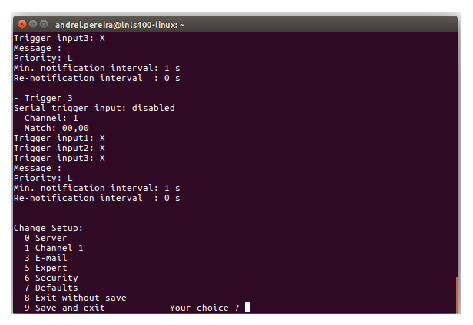
\includegraphics[width=0.7\textwidth]{telnet-image}
		\end{figure}
\FloatBarrier

	\subsection{Register Read/Write}

		\paragraph{} Both read and write operations use the same structure for the UDP data frame, which is the following:

			\bigskip
			% UDP Data Frame: byte 0-12
			\begin{tabularx}{\textwidth}{C C C C C C C C C C C C C}
			Byte 0 & Byte 1 & & & Byte 4 & Byte 5 & & & Byte 8 & Byte 9 & & & Byte 12 \\
			% fields
			\hline
			\multicolumn{1}{|c}{Command} & \multicolumn{4}{|c}{RegA} & \multicolumn{4}{|c}{RegB} & \multicolumn{4}{|c|}{RegC} \\ \hline
	    		\end{tabularx}

			\paragraph{} The \emph{RegA}, \emph{RegB}, and \emph{RegC} sections in the UDP data frame correspond to the 32-bit register sections of same name in each register. These sections carry the information to be written/read. The operation selection and register are specified by the \emph{Command} byte of the UDP data frame.

		\paragraph{Read (request)} In order to read a register, the UDP data frame \emph{Command} byte must agree with the following rule:

			\bigskip
			% Command: bits 7-0
			\begin{tabularx}{\textwidth}{C C C C C C C C}
			Bit 7 & Bit 6 & Bit 5 & Bit 4 & Bit 3 & Bit 2 & Bit 1 & Bit 0 \\
			% fields
			\hline
			\multicolumn{1}{|c}{1} & \multicolumn{1}{|c}{0} & \multicolumn{6}{|c|}{Address} \\ \hline
	    		\end{tabularx}

			\paragraph{} The first bits, from left to right, must be 1 and 0 respectively, followed by the register address.

		\paragraph{Read (response)} The response to a read request has a different \emph{Command} byte, which is represented below:

			\bigskip
			% Command: bits 7-0
			\begin{tabularx}{\textwidth}{C C C C C C C C}
			Bit 7 & Bit 6 & Bit 5 & Bit 4 & Bit 3 & Bit 2 & Bit 1 & Bit 0 \\
			% fields
			\hline
			\multicolumn{1}{|c}{1} & \multicolumn{1}{|c}{1} & \multicolumn{6}{|c|}{Address} \\ \hline
	    		\end{tabularx}		

			\paragraph{} The first bits, from left to right, must be 1 and 1 respectively, followed by the register address.

		\paragraph{Write} In order to write to a register, the UDP data frame \emph{Command} byte must agree with the following rule:

			\bigskip
			% Command: bits 7-0
			\begin{tabularx}{\textwidth}{C C C C C C C C}
			Bit 7 & Bit 6 & Bit 5 & Bit 4 & Bit 3 & Bit 2 & Bit 1 & Bit 0 \\
			% fields
			\hline
			\multicolumn{1}{|c}{0} & \multicolumn{1}{|c}{1} & \multicolumn{6}{|c|}{Address} \\ \hline
	    		\end{tabularx}
	
			\paragraph{} The first bits, from left to right, must be 0 and 1 respectively, followed by the register address.

\end{document}
\grid
